\documentclass[onecolumn]{aastex62}

\shorttitle{photon counting \& detectors}
\shortauthors{j. birky}


\begin{document}

\title{\sc Lab 1: Photon Counting \& Detectors}

\author{Jessica Birky (A13002163)}

\begin{abstract}

This example manuscript is intended to serve as a tutorial and template for
authors to use when writing their own AAS Journal articles. The manuscript
includes a history of and documents the new features in the
previous versions as well as the new features in version 6.2. This
manuscript includes many figure and table examples to illustrate these new
features.  Information on features not explicitly mentioned in the article
can be viewed in the manuscript comments or more extensive online
documentation. Authors are welcome replace the text, tables, figures, and
bibliography with their own and submit the resulting manuscript to the AAS
Journals peer review system.  The first lesson in the tutorial is to remind
authors that the AAS Journals, the Astrophysical Journal (ApJ), the
Astrophysical Journal Letters (ApJL), and Astronomical Journal (AJ), all
have a 250 word limit for the abstract.  If you exceed this length the
Editorial office will ask you to shorten it.

\end{abstract}
\bigskip

\section{Introduction} 
Photoelectric effect, CCDs, etc.

% ==================================
\section{Observations}
Nickel telescope, what are bias and flat frames


% ==================================
\section{Data Reduction \& Methods}
Poisson statistics, point to code

% ==================================
\section{Data Analysis \& Modeling}

\begin{figure}[ht]
\plotone{plots/exposure0.png}
\caption{Combined bias frames.} \label{fig:bias}
\end{figure}
\begin{figure}[ht]
\plotone{plots/exposure3.png}
\plotone{plots/exposure6.png}
\plotone{plots/exposure12.png}
\plotone{plots/exposure48.png}
\caption{Combined, bias-subtracted, flat frame histograms and images for varying exposure times (0, 3, 6, and 12 sec). \label{fig:flats1}}
\end{figure}
\begin{figure}[ht]
\plotone{plots/exposure96.png}
\plotone{plots/exposure192.png}
\plotone{plots/exposure384.png}
\plotone{plots/exposure768.png}
\caption{Combined, bias-subtracted, flat frame histograms and images for varying exposure times (96, 192, 384, and 768 sec). \label{fig:flats2}}
\end{figure}

\begin{figure}[ht]
\begin{center}
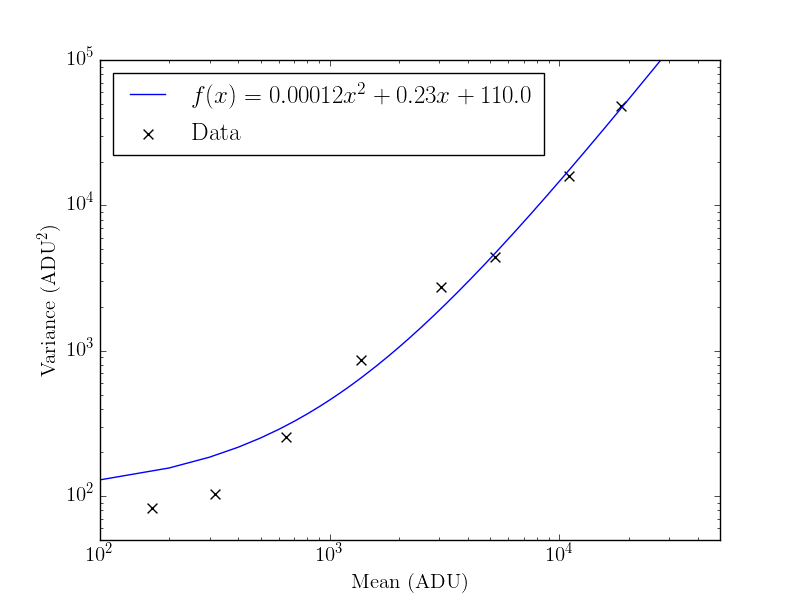
\includegraphics[width=8cm]{plots/mean_vs_variance.png}
\caption{Mean vs. variance for all bias-subtracted exposures.} \label{fig:mean_var}
\end{center}
\end{figure}

% ==================================
\section{Discussion}

% ==================================
\section{Conclusion}

% ==================================
\section{Author Contributions}

% ==================================
\section{Appendix}

\subsection{Statistics}
Mean and variance for a set of data points $x={x_1, ...,x_N}$:
\begin{equation}
	\bar{x} = \frac{1}{N} \sum^N_{i=1} x_i  
\end{equation}
\begin{equation}
	s^2 = \frac{1}{N-1} \sum^N_{i=1} (x_i - \bar{x})^2
\end{equation}

\subsection{Code}


% \begin{thebibliography}{}
% \bibitem[Astropy Collaboration et al.(2013)]{2013A&A...558A..33A} Astropy Collaboration, Robitaille, T.~P., Tollerud, E.~J., et al.\ 2013, \aap, 558, A33 
% \end{thebibliography}


\end{document}

